\section{Resultados}

\subsection{Enlaces transatlánticos}

%~ \begin{figure}[!hbp]
\begin{figure}[H]
\begin{center}
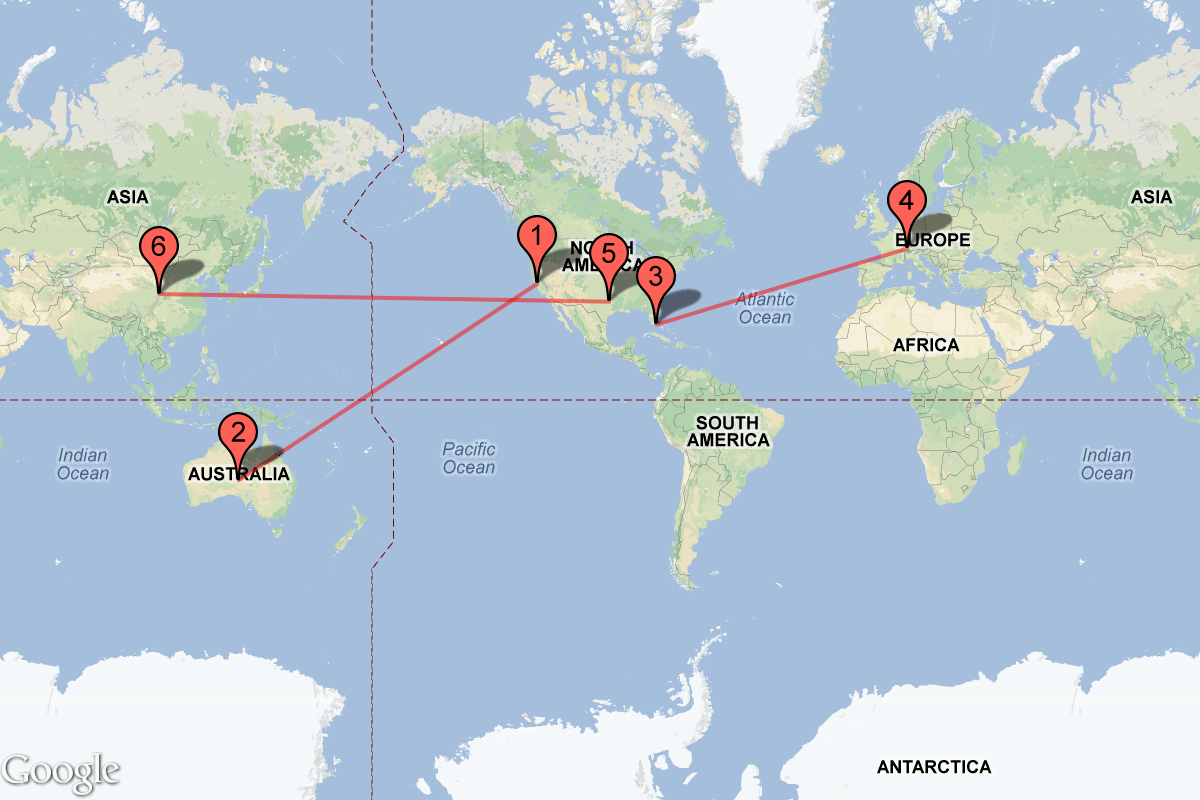
\includegraphics[width=17cm]{enlaces.png}
\end{center}
\caption{Enlaces transatlánticos} \label{figura1}
\end{figure}

\noindent \begin{center} \begin{tabular}{| c | c | c | c | c |} \hline 
Pin 	 & 	 Dirección IP 	 & 	 Coordenadas 	 & 	 Distancia total recorrida hasta él en Km 	 & 	 RTT mínimo en ms \\ \hline 
1 	 & 	 89.221.35.141 	 & 	 (37.9283,-122.0566) 	 & 	 11179.8250554 	 & 	 55.9 \\ \hline 
2 	 & 	 202.158.194.173 	 & 	 (-27.0,133.0) 	 & 	 24234.7289268 	 & 	 121.17 \\ \hline 
3 	 & 	 195.22.199.109 	 & 	 (25.7743,-80.1937) 	 & 	 7887.31191972 	 & 	 39.44 \\ \hline 
4 	 & 	 195.2.6.169 	 & 	 (47.0,8.0) 	 & 	 15702.4500297 	 & 	 78.51 \\ \hline 
5 	 & 	 89.221.40.131 	 & 	 (32.7831,-96.8067) 	 & 	 9285.34331745 	 & 	 46.43 \\ \hline 
6 	 & 	 219.158.33.189 	 & 	 (35.0,105.0) 	 & 	 21427.6048813 	 & 	 107.14 \\ \hline 
\end{tabular} \end{center}

\noindent \begin{center} \begin{tabular}{| c | c | c | c | c |} \hline 
Enlace 	 &	Distancia en Km 	& 	RTT mínimo en ms	\\ \hline 
1 - 2	 &	13054.90 	 		& 	65.27				\\ \hline 
3 - 4 	 & 	7815.13	 			& 	39.07				\\ \hline 
5 - 6 	 & 	12142.26 			&	60.71				\\ \hline 
\end{tabular} \end{center}

\subsection{Variación del RTT a lo largo del día}

\begin{figure}[H]
\begin{center}
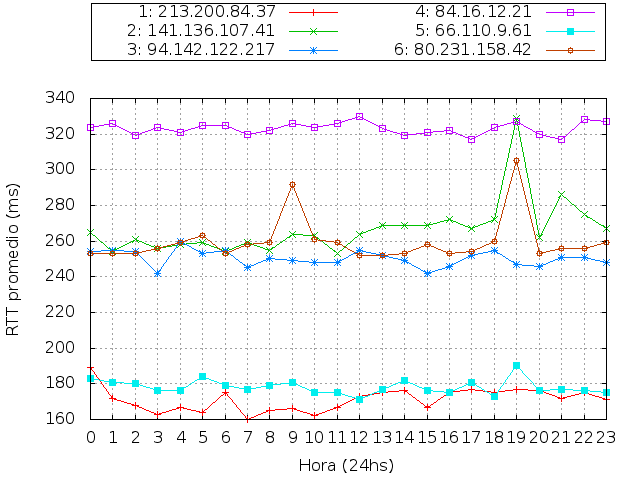
\includegraphics[width=17cm]{rtts.png}
\end{center}
\caption{Tiempo de respuesta de los enlaces transatlánticos a lo largo del día} \label{figura1}
\end{figure}

\subsection{Casos curiosos}

%~ \begin{figure}[!hbp]
\begin{figure}[H]
\begin{center}
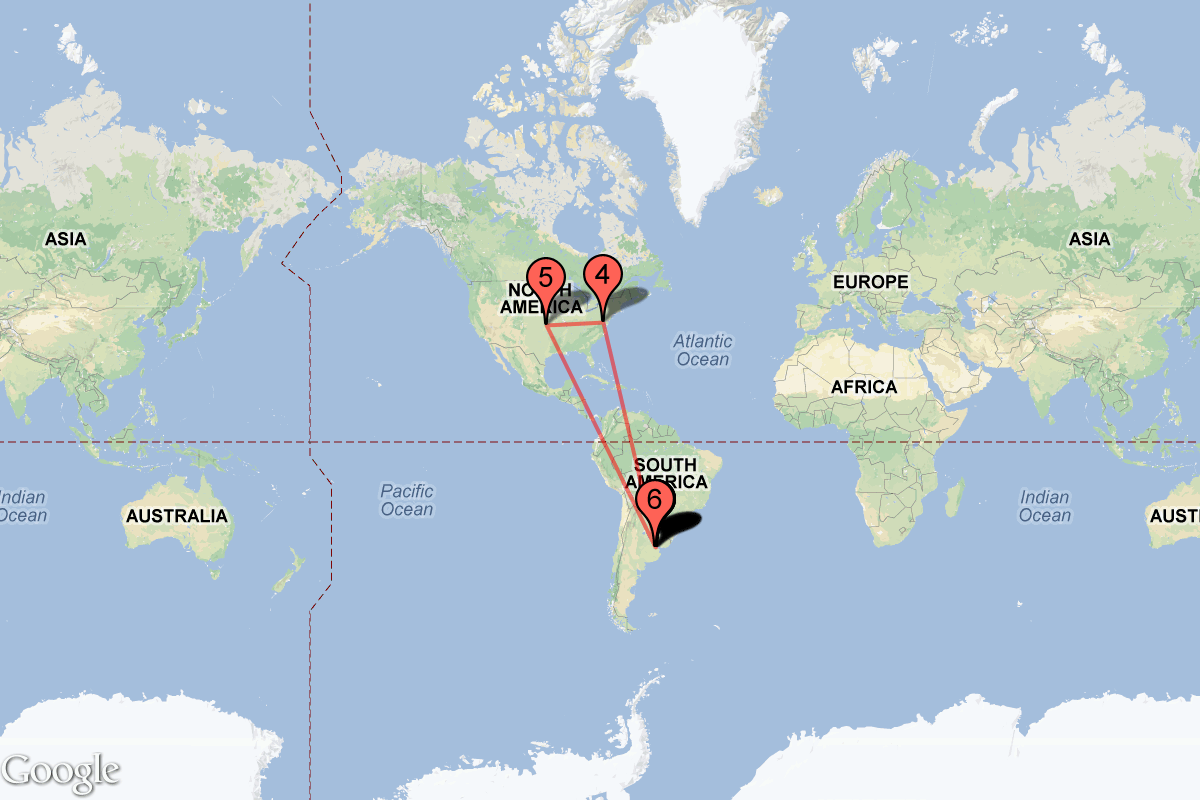
\includegraphics[width=17cm]{perfil.png}
\end{center}
\caption{Traceroute a perfil.com.ar} \label{figura1}
\end{figure}

En este caso al hacer un traceroute desde una dirección IP en Argentina a perfil.com.ar, un sitio web hosteado en Argentina, observamos que el tráfico primero se dirige a los Estados Unidos y luego vuelve al país para acceder al sitio.

\begin{figure}[H]
\begin{center}
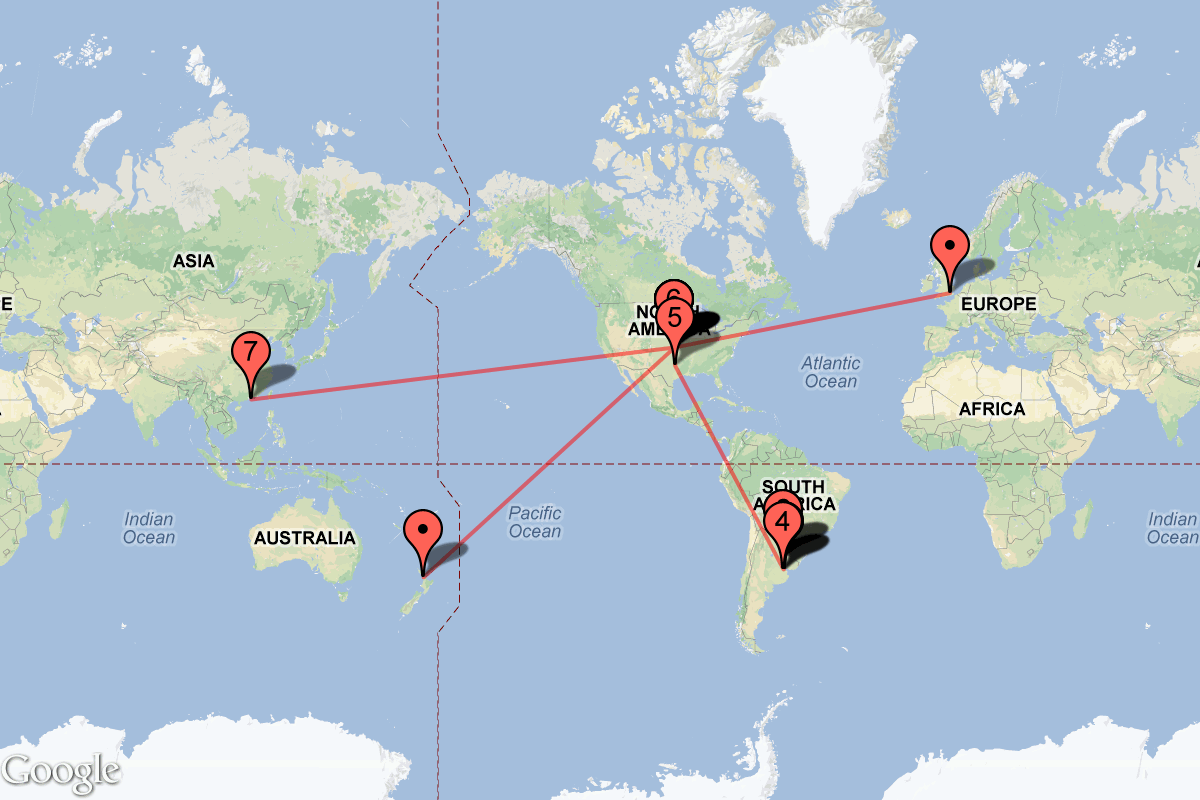
\includegraphics[width=17cm]{newzealand.png}
\end{center}
\caption{Traceroute a newzealand.govt.nz} \label{figura1}
\end{figure}

Realizamos un traceroute a una página web en Nueva Zelanda y obtuvimos que los paquetes se dirigieron primero a Estados Unidos, luego a Asia, de ahí vuelven a Norte América para dirigirse a España. Finalmente vuelven a Estados Unidos para ser enviados a Nueva Zelanda.	\\
\indent	Al intentar reproducir los resultados días más tarde no obtuvimos los mismos resultados, en una ocasión iba directo desde Estados Unidos y en otras fue a través de Asia.
